\documentclass[12pt]{report}

% ── Packages ─────────────────────────────────────────────────────────────────
\usepackage{parskip}
\setlength{\parindent}{2em}

\usepackage[a4paper, margin=1in]{geometry}
\usepackage{amsmath,amssymb,amsfonts}
\usepackage{amsthm}
\usepackage{mathrsfs}
\usepackage{hyperref}
\usepackage{tikz}
\usetikzlibrary{arrows.meta, positioning, shapes.geometric, arrows}
\usepackage{longtable}
\usepackage{forest}
\usepackage{graphicx}
\usepackage{listings}
\usepackage{xcolor}
\usepackage{caption}
\usepackage{fancyhdr}
\usepackage{float}
\usepackage{multirow}
\usepackage[title]{appendix}
\usepackage{textcomp}
\usepackage{booktabs}
\usepackage{array}
\usepackage{algorithm}
\usepackage{algorithmicx}
\usepackage{algpseudocode}

% ── Colours ───────────────────────────────────────────────────────────────────
\definecolor{codegray}{rgb}{0.4,0.4,0.4}
\definecolor{codeblue}{rgb}{0.0,0.0,0.8}
\definecolor{codegreen}{rgb}{0.0,0.5,0.0}
\definecolor{codered}{rgb}{0.6,0.0,0.0}
\definecolor{codebg}{RGB}{235,245,255}

% ── TikZ styles ───────────────────────────────────────────────────────────────
\tikzstyle{startstop} = [rectangle, rounded corners, minimum width=3cm,
    minimum height=1cm, text centered, draw=black, fill=blue!20]
\tikzstyle{process}   = [rectangle, minimum width=3cm, minimum height=1cm,
    text centered, draw=black, fill=yellow!30]
\tikzstyle{arrow}     = [thick,->,>=stealth, draw=red]

% ── Listings styles ───────────────────────────────────────────────────────────
\lstdefinestyle{cpp}{
    language=C++,
    backgroundcolor=\color{codebg},
    basicstyle=\ttfamily\footnotesize,
    keywordstyle=\color{codeblue}\bfseries,
    commentstyle=\color{codegreen},
    stringstyle=\color{codered},
    numbers=left,
    numberstyle=\tiny\color{codegray},
    stepnumber=1,
    numbersep=8pt,
    breaklines=true,
    frame=single,
    captionpos=b,
    showstringspaces=false,
    tabsize=2,
}
\lstdefinestyle{python}{
    language=Python,
    backgroundcolor=\color{codebg},
    basicstyle=\ttfamily\footnotesize,
    keywordstyle=\color{codeblue}\bfseries,
    commentstyle=\color{codegreen},
    stringstyle=\color{codered},
    numbers=left,
    numberstyle=\tiny\color{codegray},
    stepnumber=1,
    numbersep=8pt,
    breaklines=true,
    frame=single,
    captionpos=b,
    showstringspaces=false,
    tabsize=2,
}
\lstdefinestyle{typescript}{
    language=Java,
    backgroundcolor=\color{codebg},
    basicstyle=\ttfamily\footnotesize,
    keywordstyle=\color{codeblue}\bfseries,
    commentstyle=\color{codegreen},
    stringstyle=\color{codered},
    numbers=left,
    numberstyle=\tiny\color{codegray},
    stepnumber=1,
    numbersep=8pt,
    breaklines=true,
    frame=single,
    captionpos=b,
    showstringspaces=false,
    tabsize=2,
    morekeywords={const,let,async,await,export,import,type,from,
                  interface,null,undefined,string,number,boolean},
}

% ── Header / Footer ───────────────────────────────────────────────────────────
\pagestyle{fancy}
\fancyhf{}
\rhead{EE-427 Mini Project}
\lhead{Voice-Controlled Robot Car}
\rfoot{\thepage}

% ── Hyperref ─────────────────────────────────────────────────────────────────
\hypersetup{colorlinks=true, linkcolor=black, urlcolor=blue, citecolor=black}

\newcommand{\indentpar}{\hspace*{2em}}

% ─────────────────────────────────────────────────────────────────────────────
\begin{document}
\pagenumbering{gobble}

% ── Title Page ───────────────────────────────────────────────────────────────
\begin{titlepage}
    \centering
    \Large \textbf{Mini Project Report}\\[0.2cm]
    \Large{of}\\[0.3cm]
    \Huge \textbf{Voice-Controlled Robot Car:\\[0.3cm]An IoT Solution}\\[0.5cm]
    \large{Submitted in Fulfilment of the Course}\\[0.2cm]
    \large\textbf{EE-427 Computer Networks}\\[0.5cm]

    \Large{Submitted by}\\[0.4cm]
    \large\textbf{
        Suyash D Nahar \hfill (231EE257)\\[0.15cm]
        Thakkar Vanshi Ramesh \hfill (231EE259)\\[0.15cm]
        Tridhatri Prakash \hfill (231EE260)\\[0.15cm]
        Venkatesh S \hfill (231EE262)\\[0.15cm]
        Vijeeth J Poojary \hfill (231EE263)
    }\\[0.6cm]

    \small{Under the Guidance of}\\[0.3cm]
    \large\textbf{Dr.\ K.\ P.\ Vittal}\\
    \small{Professor, Department of Electrical and Electronics Engineering}\\[0.4cm]

    \small{To}\\[0.3cm]
    \small{Department of Electrical and Electronics Engineering}\\
    \small{of}\\
    \small{Bachelor of Technology in Electrical and Electronics Engineering}\\[0.5cm]

    \includegraphics[width=4cm]{nitk.png}\par\vspace{0.5cm}

    \large\textbf{DEPARTMENT OF ELECTRICAL AND ELECTRONICS ENGINEERING}\\[0.4cm]
    \large\textbf{NATIONAL INSTITUTE OF TECHNOLOGY KARNATAKA}\\
    \large\textbf{SURATHKAL, MANGALURU -- 575025}\\[0.4cm]
    {\large\textbf{April 2025}\par}
\end{titlepage}

% ─────────────────────────────────────────────────────────────────────────────
\pagenumbering{roman}

% ── Acknowledgement ──────────────────────────────────────────────────────────
\chapter*{Acknowledgement}
\addcontentsline{toc}{chapter}{Acknowledgement}

We express our profound gratitude and deep regard to
\textbf{Dr.\ K.\ P.\ Vittal (Professor, Department of Electrical and Electronics
Engineering, NITK Surathkal)} for his guidance, valuable feedback, and constant
encouragement throughout this project. His insightful suggestions on network
protocol design and IoT architecture were instrumental in shaping the final
system.

We are also grateful to the \textbf{Department of Electrical and Electronics
Engineering}, National Institute of Technology Karnataka, Surathkal, for providing
the necessary resources and facilities to complete this project.

\vspace{1cm}
\hfill Surathkal, Mangaluru -- 575\,025\\
\hfill April 2025

% ── Table of Contents ────────────────────────────────────────────────────────
\tableofcontents
\newpage

% ── Abstract ─────────────────────────────────────────────────────────────────
\chapter*{Abstract}
\addcontentsline{toc}{chapter}{Abstract}

The rapid proliferation of smart devices and the Internet of Things (IoT) has
expanded the scope of remote control applications beyond local networks to
internet-scale deployments. This project demonstrates an end-to-end IoT system
for the Wi-Fi control of a four-wheeled robot car using an ESP32 microcontroller,
with three independent control interfaces: voice commands via the browser-native
Web Speech API, a graphical D-pad, and a Python keyboard controller.

Motion commands (forward, backward, left, right, stop) and speed levels (LOW,
MED, HIGH) are transmitted from a React frontend hosted on Vercel through a
secure FastAPI bridge server tunnelled over ngrok to the ESP32 on the local
network. The architecture illustrates key computer networking concepts including
HTTP/REST, TLS~1.3, CORS, API key authentication, NAT traversal via reverse
tunnelling, and the full OSI protocol stack across both internet and LAN segments.

The system was successfully demonstrated with real hardware, achieving
sub-300\,ms round-trip latency from voice utterance to motor actuation under
normal network conditions. The deployed frontend is publicly accessible at
\url{https://ee427-robot.vercel.app}.

% ─────────────────────────────────────────────────────────────────────────────
\pagenumbering{arabic}

\chapter{Introduction}

The Internet of Things (IoT) has become a transformative paradigm enabling
physical devices to be monitored and controlled over internet-scale networks.
Modern IoT deployments require the integration of embedded hardware, network
protocol stacks, cloud hosting, and user interface design into a cohesive system.
This project implements all four layers in the context of a remotely controlled
robot car.

The core hardware is an ESP32 microcontroller, which connects to a local Wi-Fi
network and hosts a lightweight HTTP server. An L298N dual H-bridge motor driver
translates digital GPIO signals and PWM output from the ESP32 into mechanical
motion across four DC gear motors. The system supports four directions of
movement and three discrete speed levels (LOW, MED, HIGH) controlled via PWM
duty cycle.

Internet connectivity is achieved through a three-tier software architecture:
\begin{enumerate}
    \item A \textbf{React frontend} deployed on Vercel accepts user input
          through voice recognition or manual D-pad controls.
    \item A \textbf{FastAPI bridge server} running on the local machine
          authenticates requests with an API key and relays commands to the
          ESP32 over the LAN.
    \item An \textbf{ngrok reverse tunnel} provides a stable public HTTPS
          endpoint for the bridge server, enabling the Vercel-hosted frontend
          to reach the LAN device through NAT and firewalls.
\end{enumerate}

This project provides practical exposure to REST API design, HTTP/HTTPS mechanics,
TLS termination, CORS policy enforcement, NAT traversal, and the mapping of
application-layer commands through the OSI protocol stack to physical motor
actuation --- directly addressing the curriculum objectives of EE-427 Computer
Networks.

\chapter{Methodology}

\section{Software Tools Used}

\begin{itemize}
    \item \textbf{Arduino IDE}: Development environment for writing and flashing
          C++ firmware to the ESP32. Configures Wi-Fi station (STA) mode,
          instantiates the \texttt{WebServer} class on port 80, and registers
          eight HTTP route handlers for motion and speed commands.

    \item \textbf{FastAPI (Python)}: Lightweight ASGI web framework for the bridge
          server. Handles \texttt{X-Api-Key} header authentication, validates
          JSON request bodies using Pydantic models, and forwards commands to the
          ESP32 via a persistent \texttt{requests.Session}.

    \item \textbf{React + Vite (TypeScript)}: Frontend framework for the control
          UI. Implements voice recognition using the browser-native
          \texttt{SpeechRecognition} API, a D-pad for manual control, and speed
          selector buttons (LOW / MED / HIGH).

    \item \textbf{Vercel}: Cloud platform hosting the React frontend as a static
          site with global CDN distribution. Build-time environment variables
          (\texttt{VITE\_API\_URL}, \texttt{VITE\_API\_KEY}) configure the API
          endpoint and authentication key.

    \item \textbf{ngrok}: Reverse tunnelling service exposing the locally running
          FastAPI server (port 8000) as a public HTTPS endpoint. Performs TLS
          termination at the edge, enabling secure communication from the
          internet to the LAN bridge server.

    \item \textbf{Web Speech API}: Browser-native speech recognition API
          (available in Chrome and Edge) that provides continuous transcription
          of voice input. Interim and final results are processed with
          regular-expression pattern matching; an 800\,ms time-based debounce
          prevents duplicate command firings.

    \item \textbf{pynput}: Python library used in the standalone keyboard
          controller (\texttt{esp32\_controller.py}) to capture keyboard events
          non-blockingly. WASD keys map to directional commands; keys 1/2/3 set
          speed levels, bypassing the browser and ngrok entirely.

    \item \textbf{uvicorn}: ASGI server used to run the FastAPI application
          locally on port 8000.
\end{itemize}

\section{Hardware Tools Used}

\begin{itemize}
    \item \textbf{ESP32 Microcontroller}: Dual-core 32-bit Xtensa LX6 processor
          with integrated 802.11 b/g/n Wi-Fi (2.4\,GHz only). Operates in
          station (STA) mode, connects to the local router, and hosts an HTTP
          server on port 80. The LEDC (LED Control) PWM peripheral generates
          motor speed signals.

    \item \textbf{L298N Motor Driver}: Dual H-bridge module capable of driving two
          DC motors simultaneously. Speed is regulated via PWM on the enable pins
          (ENA, ENB); direction is controlled via input pins (IN1--IN4). The
          module includes an onboard 5\,V regulator for logic supply.

    \item \textbf{4$\times$ DC Gear Motors}: Provide mechanical drive to each
          wheel. Speed is proportional to PWM duty cycle: LOW\,=\,100/255
          ($\approx$39\%), MED\,=\,175/255 ($\approx$69\%), HIGH\,=\,255/255
          (100\%).

    \item \textbf{18650 Li-Ion Battery Pack (2S)}: Two 3.7\,V cells in series
          providing $\approx$7.4\,V nominal to the L298N motor driver VCC input.
          The ESP32 is powered separately via USB during development.

    \item \textbf{Acrylic 4-Wheel Robot Chassis}: Transparent acrylic frame with
          four motor mounts housing the drive train, motor driver, battery pack,
          and ESP32.

    \item \textbf{Jumper Wires and Connectors}: Connect ESP32 GPIO pins to L298N
          input/enable pins and the battery pack to the motor driver power rails.
\end{itemize}

\chapter{Network Architecture}

The system follows a three-tier IoT architecture spanning the public internet and
a private LAN, as shown in Figure~\ref{fig:sequence}.

\section{System Tiers}

\textbf{Tier 1 --- Edge Device (ESP32 on LAN):}
The ESP32 connects to the home router in station mode, assigned IP address
\texttt{192.168.1.192}. It hosts an HTTP server on port 80 responding to the
routes listed in Table~\ref{tab:routes}.

\begin{table}[H]
    \centering
    \begin{tabular}{ll}
        \toprule
        \textbf{Route} & \textbf{Action} \\
        \midrule
        \texttt{GET /F}        & Drive forward \\
        \texttt{GET /B}        & Drive backward \\
        \texttt{GET /L}        & Turn left \\
        \texttt{GET /R}        & Turn right \\
        \texttt{GET /S}        & Stop (PWM = 0, dynamic braking) \\
        \texttt{GET /SPD/LOW}  & Set speed to LOW (PWM 100/255) \\
        \texttt{GET /SPD/MED}  & Set speed to MED (PWM 175/255) \\
        \texttt{GET /SPD/HIGH} & Set speed to HIGH (PWM 255/255) \\
        \bottomrule
    \end{tabular}
    \caption{ESP32 HTTP API route table.}
    \label{tab:routes}
\end{table}

\textbf{Tier 2 --- Bridge Server (FastAPI on Mac):}
A FastAPI server on the same LAN machine authenticates all incoming requests via
the \texttt{X-Api-Key} HTTP header matched against the \texttt{BRIDGE\_API\_KEY}
environment variable. It validates the command body using Pydantic, then forwards
a \texttt{GET} request to the ESP32. A persistent \texttt{requests.Session} with
configurable connect/read timeouts is used. Read timeouts from the ESP32 (which
may occur when the motor command blocks the firmware's response loop) are handled
gracefully: the server returns \texttt{\{"ok":true, "esp\_warning":"read\_timeout"\}}
rather than a 502 error, since the command typically executes regardless.

An ngrok agent forwards public HTTPS traffic on the ngrok subdomain to
\texttt{localhost:8000}, providing TLS~1.3 termination and NAT traversal without
requiring any router port-forwarding.

\textbf{Tier 3 --- Frontend (React on Vercel):}
The React application, built with Vite and TypeScript, is deployed to Vercel's
global CDN and publicly accessible at \url{https://ee427-robot.vercel.app}.
It communicates with the bridge server exclusively over HTTPS, including the
\texttt{ngrok-skip-browser-warning} header to bypass the ngrok free-tier
interstitial page.

\begin{figure}[H]
    \centering
    
\includegraphics[width=\textwidth]{diagram.png}
    \caption{End-to-end message sequence diagram showing a motion command,
             a speed change, and the keyboard controller path which bypasses
             the internet entirely.}
    \label{fig:sequence}
\end{figure}

\section{OSI Layer Mapping}

Table~\ref{tab:osi} maps the command path across the OSI protocol stack for
both network segments --- the internet-facing path (Browser to ngrok) and the
LAN path (FastAPI to ESP32).

\begin{table}[H]
    \centering
    \renewcommand{\arraystretch}{1.3}
    \begin{tabular}{p{1.6cm}p{4.5cm}p{4.5cm}}
        \toprule
        \textbf{Layer} &
        \textbf{Browser $\rightarrow$ ngrok (Internet)} &
        \textbf{FastAPI $\rightarrow$ ESP32 (LAN)} \\
        \midrule
        7 App     & HTTPS POST \texttt{/api/command} JSON
                  & HTTP GET \texttt{/F}, plain-text response \\
        6 Pres    & TLS 1.3 encryption; JSON serialisation
                  & No encryption; ASCII text \\
        5 Session & HTTP/1.1 keep-alive
                  & \texttt{requests.Session} connection reuse \\
        4 Trans   & TCP; dst port 443
                  & TCP; dst port 80; 2\,s connect timeout \\
        3 Network & Internet routing via BGP; DNS lookup
                  & 192.168.1.0/24 subnet; ARP MAC resolution \\
        2 Link    & 802.11 Wi-Fi / Ethernet MAC frames
                  & 802.11 2.4\,GHz Wi-Fi MAC frames \\
        1 Phys    & RF / copper / fibre (ISP uplink)
                  & 2.4\,GHz RF; ESP32 ceramic antenna \\
        \bottomrule
    \end{tabular}
    \caption{OSI layer mapping across both network segments.}
    \label{tab:osi}
\end{table}

\section{Execution Flow}

Figure~\ref{fig:flow} shows the high-level execution flow from user input to
motor actuation.

\begin{figure}[H]
\centering
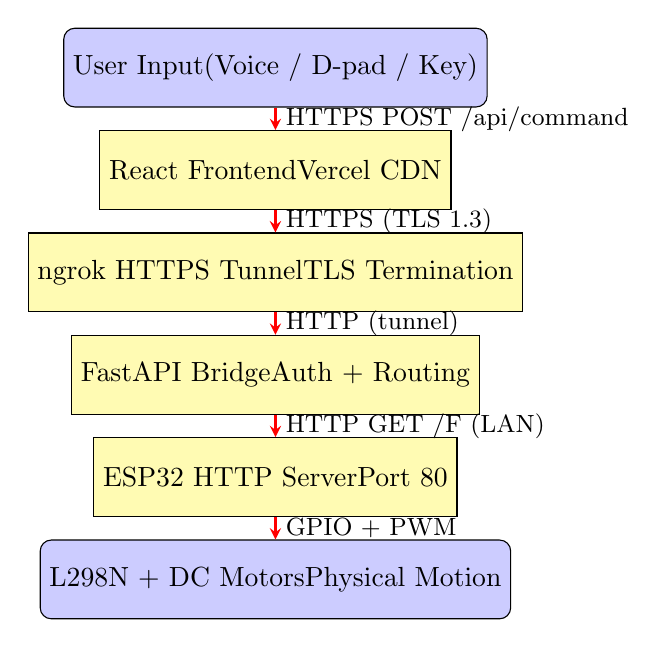
\begin{tikzpicture}[node distance=1.3cm]
    \node (user)  [startstop]                         {User Input\\(Voice / D-pad / Key)};
    \node (react) [process, below of=user]            {React Frontend\\Vercel CDN};
    \node (ngrok) [process, below of=react]           {ngrok HTTPS Tunnel\\TLS Termination};
    \node (api)   [process, below of=ngrok]           {FastAPI Bridge\\Auth + Routing};
    \node (esp)   [process, below of=api]             {ESP32 HTTP Server\\Port 80};
    \node (motor) [startstop, below of=esp]           {L298N + DC Motors\\Physical Motion};

    \draw [arrow] (user)  -- node[right]{\small HTTPS POST /api/command} (react);
    \draw [arrow] (react) -- node[right]{\small HTTPS (TLS 1.3)} (ngrok);
    \draw [arrow] (ngrok) -- node[right]{\small HTTP (tunnel)} (api);
    \draw [arrow] (api)   -- node[right]{\small HTTP GET /F (LAN)} (esp);
    \draw [arrow] (esp)   -- node[right]{\small GPIO + PWM} (motor);
\end{tikzpicture}
\caption{Execution flow from user input to motor actuation.}
\label{fig:flow}
\end{figure}

\chapter{Implementation}

\section{Hardware Configuration}

The L298N motor driver is connected to the ESP32 as follows:
direction pins IN1/IN2 drive the left motor pair; IN3/IN4 drive the right motor
pair. Enable pins ENA and ENB receive PWM signals from the ESP32 LEDC peripheral
(channels 0 and 1 respectively). The 7.4\,V battery pack powers the L298N VCC;
the onboard 5\,V regulator supplies logic power to the L298N. The ESP32 GPIO
outputs (3.3\,V) are directly compatible with the L298N logic inputs.

\begin{figure}[H]
    \centering
    \includegraphics[width=0.72\textwidth]{robot_hardware.jpg}
    \caption{Top view of the robot car: ESP32 (right), L298N motor driver
             (centre, red board), and 18650 Li-Ion battery pack (left) mounted
             on the acrylic chassis.}
    \label{fig:hardware}
\end{figure}

\section{ESP32 Firmware}

The firmware is written in C++ using the Arduino framework for ESP32.
On startup, the ESP32 connects to the configured Wi-Fi network in station mode
and prints its assigned IP address to the serial console at 115200 baud.
Eight route handlers are registered with the \texttt{WebServer} object before
calling \texttt{server.begin()}.

Speed is maintained as a global integer \texttt{gSpeed} (0--255) updated by the
\texttt{/SPD/*} route handlers. Motion handlers set the H-bridge direction pins
via \texttt{digitalWrite()} and call \texttt{ledcWrite()} with the current
\texttt{gSpeed} value on both PWM channels simultaneously, ensuring symmetric
drive on all four wheels.

The stop handler (\texttt{/S}) drives all direction pins LOW and sets PWM to
zero, applying dynamic braking by shorting the motor terminals through the
H-bridge.

\section{FastAPI Bridge Server}

The bridge server exposes two authenticated POST endpoints:

\begin{itemize}
    \item \textbf{\texttt{POST /api/command}}: Accepts JSON body
          \texttt{\{cmd: "forward"|"backward"|"left"|"right"|"stop"\}},
          maps the command string to an ESP32 route letter via a dictionary,
          and issues \texttt{GET /\{letter\}} to the ESP32.

    \item \textbf{\texttt{POST /api/speed}}: Accepts
          \texttt{\{speed: "LOW"|"MED"|"HIGH"\}} and issues
          \texttt{GET /SPD/\{level\}} to the ESP32.
\end{itemize}

CORS is configured via the \texttt{CORS\_ORIGINS} environment variable
(comma-separated list of allowed origins), supporting both the Vercel production
URL and any preview deployment subdomains. All sensitive values are stored in a
\texttt{.env} file loaded at startup via \texttt{python-dotenv}.

\section{React Frontend}

The frontend provides three control modes operating over the same API:

\begin{enumerate}
    \item \textbf{Voice Control}: Uses the browser \texttt{SpeechRecognition}
          API in continuous mode with interim results enabled. Only finalised
          transcript segments trigger command matching via the
          \texttt{transcriptToCommand()} function. Matched keywords:
          \textit{forward}/\textit{front}, \textit{back}/\textit{backward},
          \textit{left}, \textit{right}, \textit{stop},
          \textit{faster}/\textit{fast} (speed $+$1 step),
          \textit{slower}/\textit{slow} (speed $-$1 step). An 800\,ms
          time-based debounce prevents duplicate commands from repeated
          recognition events.

    \item \textbf{D-pad (Manual)}: Five buttons in a cross arrangement send
          direct drive commands via \texttt{POST /api/command}. A central stop
          button halts the robot.

    \item \textbf{Speed Control}: Three buttons (LOW / MED / HIGH) send
          \texttt{POST /api/speed}. The active level is visually highlighted.
          Voice speed commands adjust the level relatively by $\pm$1 step using
          a \texttt{useRef} mirror of the speed state, avoiding stale closure
          issues in the voice callback.
\end{enumerate}

\begin{figure}[H]
    \centering
    \includegraphics[width=0.44\textwidth]{robot_demo.jpg}
    \caption{Live demonstration: the deployed web application running on a
             mobile browser controlling the robot car. Voice transcript
             ``forward'' is visible; LOW speed is active.}
    \label{fig:demo}
\end{figure}

\section{Keyboard Controller}

A standalone Python script (\texttt{esp32\_controller.py}) provides direct LAN
control without requiring a browser or ngrok. Using \texttt{pynput} for
non-blocking keyboard event capture:

\begin{center}
\begin{tabular}{ll}
    \toprule
    \textbf{Key} & \textbf{Action} \\
    \midrule
    W & Forward (\texttt{GET /F}) \\
    S & Backward (\texttt{GET /B}) \\
    A & Left (\texttt{GET /L}) \\
    D & Right (\texttt{GET /R}) \\
    E & Stop (\texttt{GET /S}) \\
    1 & Speed LOW (\texttt{GET /SPD/LOW}) \\
    2 & Speed MED (\texttt{GET /SPD/MED}) \\
    3 & Speed HIGH (\texttt{GET /SPD/HIGH}) \\
    Q & Quit (sends stop first) \\
    \bottomrule
\end{tabular}
\end{center}

This path bypasses all internet-facing components, reducing round-trip latency
to a single LAN HTTP hop ($<$5\,ms typical).

\section{Modes of Operation}

\begin{table}[H]
    \centering
    \renewcommand{\arraystretch}{1.2}
    \begin{tabular}{p{2.2cm}p{2.8cm}p{7cm}}
        \toprule
        \textbf{Mode} & \textbf{Input} & \textbf{Network Path} \\
        \midrule
        Voice      & Chrome / Edge browser
                   & Browser $\to$ Vercel $\to$ ngrok $\to$ FastAPI $\to$ ESP32 \\
        D-pad      & Any browser / device
                   & Browser $\to$ Vercel $\to$ ngrok $\to$ FastAPI $\to$ ESP32 \\
        Keyboard   & Terminal (WASD + 1/2/3)
                   & Python script $\to$ ESP32 direct (LAN only, no ngrok) \\
        Speed btn  & Browser buttons
                   & Browser $\to$ Vercel $\to$ ngrok $\to$ FastAPI $\to$ ESP32 \\
        Speed voice& \textit{faster / slower}
                   & Same path as voice \\
        \bottomrule
    \end{tabular}
    \caption{Summary of control modes and their network paths.}
    \label{tab:modes}
\end{table}

\chapter{Results and Discussion}

The system was successfully demonstrated on physical hardware. The following
performance characteristics and observations were recorded.

\section{Latency Measurements}

\begin{itemize}
    \item \textbf{Voice-to-motor latency}: 200--400\,ms from utterance to wheel
          movement. This is dominated by speech recognition finalisation
          ($\approx$150--300\,ms) rather than the network round-trip, as the
          Web Speech API buffers audio before emitting a final result.

    \item \textbf{API round-trip time}: 180--250\,ms average for the full HTTPS
          round trip (Vercel $\to$ ngrok $\to$ FastAPI $\to$ ESP32 $\to$ return)
          on a home broadband connection.

    \item \textbf{Keyboard controller latency}: $<$5\,ms for a direct LAN HTTP
          request to the ESP32, confirming that internet-facing components
          contribute the majority of the overall latency.
\end{itemize}

\section{Challenges and Solutions}

\begin{itemize}
    \item \textbf{CORS policy enforcement}: The Vercel platform generates two
          distinct URLs per project --- a stable production URL
          (\texttt{ee427-robot.vercel.app}) and a deployment-specific preview
          URL. Both must be added to \texttt{CORS\_ORIGINS} in the backend
          \texttt{.env} file. Additionally, trailing slashes in origin strings
          cause CORS mismatch failures, as the comparison is exact-string.

    \item \textbf{ESP32 read timeouts}: The ESP32 firmware occasionally delayed
          HTTP responses while executing motor commands. The bridge server was
          updated to distinguish read timeouts (command executed, no response
          body) from connect timeouts (ESP32 unreachable). Read timeouts return
          \texttt{\{"ok":true, "esp\_warning":"read\_timeout"\}} to prevent false
          502 errors appearing in the frontend.

    \item \textbf{ngrok subdomain rotation}: The free ngrok tier assigns a new
          random subdomain on each tunnel restart, requiring a
          \texttt{VITE\_API\_URL} update and Vercel redeploy. Registering a
          static ngrok domain (available free with account verification)
          eliminates this step.

    \item \textbf{Voice recognition deduplication}: The initial implementation
          used the transcript string as a deduplication key, causing the same
          command to fire only once even after a pause. This was replaced with
          a time-based debounce (800\,ms window), allowing natural repeated
          commands while filtering rapid duplicates from continuous recognition.
\end{itemize}

\section{Speed Control Results}

The three PWM duty cycle levels produced clearly distinguishable mechanical
speeds:

\begin{itemize}
    \item \textbf{LOW} (100/255, $\approx$39\%): Precise slow-speed manoeuvring;
          suitable for indoor navigation in confined spaces.
    \item \textbf{MED} (175/255, $\approx$69\%): Default operating speed;
          good balance of control and responsiveness.
    \item \textbf{HIGH} (255/255, 100\%): Maximum speed; suitable for open
          spaces but reduced control precision.
\end{itemize}

\chapter{Conclusion}

This project successfully demonstrates the design and implementation of an
IoT-based remote control system for a four-wheeled robot car using the ESP32
microcontroller, bridging a private LAN device to the public internet through a
FastAPI bridge server and ngrok reverse tunnel. Three independent control
modes --- voice recognition, graphical D-pad, and keyboard controller --- were
implemented and tested on real hardware, all converging on the same REST HTTP API
exposed by the ESP32 firmware.

The architecture addresses real-world IoT deployment challenges: API key
authentication for security, CORS policy configuration for cross-origin browser
access, graceful handling of ESP32 read timeouts, and NAT traversal without
router configuration through reverse tunnelling. The system complies with
modern IoT standards by using HTTPS for all internet-facing communication,
structured JSON payloads, and environment-variable-based configuration.

The project demonstrates the full network stack in practice: REST API design at
the application layer, TLS 1.3 encryption at the presentation layer, persistent
TCP session management at the transport layer, IP routing and ARP at the network
and data-link layers, and 802.11 Wi-Fi radio at the physical layer. The modular
three-tier architecture (ESP32 firmware / FastAPI bridge / React frontend) is
directly extensible to other IoT control scenarios, including the ceiling fan
speed controller described in the project specification.

% ─────────────────────────────────────────────────────────────────────────────
\begin{thebibliography}{99}

\bibitem{esp32}
Espressif Systems,
\textit{ESP32 Technical Reference Manual},
Espressif Systems, 2023.
[Online]. Available:
\url{https://www.espressif.com/sites/default/files/documentation/esp32_technical_reference_manual_en.pdf}

\bibitem{arduino-esp32}
Espressif Systems,
\textit{Arduino Core for the ESP32},
2024.
[Online]. Available: \url{https://docs.espressif.com/projects/arduino-esp32/en/latest/}.
Accessed: April 2025.

\bibitem{fastapi}
S. Ramirez,
\textit{FastAPI Documentation},
2024.
[Online]. Available: \url{https://fastapi.tiangolo.com/}.
Accessed: April 2025.

\bibitem{webspeech}
MDN Web Docs,
\textit{Web Speech API},
Mozilla Developer Network, 2024.
[Online]. Available:
\url{https://developer.mozilla.org/en-US/docs/Web/API/Web_Speech_API}.
Accessed: April 2025.

\bibitem{ngrok}
ngrok Inc.,
\textit{ngrok Documentation},
2024.
[Online]. Available: \url{https://ngrok.com/docs}.
Accessed: April 2025.

\bibitem{vercel}
Vercel Inc.,
\textit{Vercel Documentation},
2024.
[Online]. Available: \url{https://vercel.com/docs}.
Accessed: April 2025.

\bibitem{rfc7231}
R. Fielding and J. Reschke,
\textit{RFC 7231: Hypertext Transfer Protocol (HTTP/1.1): Semantics and Content},
IETF, 2014.
[Online]. Available: \url{https://tools.ietf.org/html/rfc7231}

\bibitem{rfc8446}
E. Rescorla,
\textit{RFC 8446: The Transport Layer Security (TLS) Protocol Version 1.3},
IETF, 2018.
[Online]. Available: \url{https://tools.ietf.org/html/rfc8446}

\end{thebibliography}

% ─────────────────────────────────────────────────────────────────────────────
\newpage
\chapter*{Source Code}
\addcontentsline{toc}{chapter}{Source Code}

\section*{Listing 1: ESP32 Firmware (Arduino C++)}

\begin{lstlisting}[style=cpp,
caption={ESP32 firmware --- Wi-Fi HTTP server with motion and speed control.}]
#include <WiFi.h>
#include <WebServer.h>

const char* WIFI_SSID     = "YOUR_SSID";
const char* WIFI_PASSWORD = "YOUR_PASSWORD";

// L298N pins
#define IN1 12    // Left motor direction A
#define IN2 13    // Left motor direction B
#define IN3 25    // Right motor direction A
#define IN4 26    // Right motor direction B
#define ENA 14    // Left PWM  (LEDC channel 0)
#define ENB 27    // Right PWM (LEDC channel 1)

const int PWM_FREQ = 1000;
const int PWM_RES  = 8;      // 0-255
int       gSpeed   = 175;    // default: MED

WebServer server(80);

void setMotor(int a, int b, int c, int d, int spd) {
  digitalWrite(IN1,a); digitalWrite(IN2,b);
  digitalWrite(IN3,c); digitalWrite(IN4,d);
  ledcWrite(0,spd);    ledcWrite(1,spd);
}

void handleForward()  { setMotor(1,0,1,0,gSpeed);
                        server.send(200,"text/plain","F"); }
void handleBackward() { setMotor(0,1,0,1,gSpeed);
                        server.send(200,"text/plain","B"); }
void handleLeft()     { setMotor(0,1,1,0,gSpeed);
                        server.send(200,"text/plain","L"); }
void handleRight()    { setMotor(1,0,0,1,gSpeed);
                        server.send(200,"text/plain","R"); }
void handleStop()     { setMotor(0,0,0,0,0);
                        server.send(200,"text/plain","S"); }
void handleSpdLow()   { gSpeed=100;
                        server.send(200,"text/plain","SPD:LOW"); }
void handleSpdMed()   { gSpeed=175;
                        server.send(200,"text/plain","SPD:MED"); }
void handleSpdHigh()  { gSpeed=255;
                        server.send(200,"text/plain","SPD:HIGH"); }

void setup() {
  Serial.begin(115200);
  pinMode(IN1,OUTPUT); pinMode(IN2,OUTPUT);
  pinMode(IN3,OUTPUT); pinMode(IN4,OUTPUT);
  ledcSetup(0,PWM_FREQ,PWM_RES); ledcAttachPin(ENA,0);
  ledcSetup(1,PWM_FREQ,PWM_RES); ledcAttachPin(ENB,1);

  WiFi.begin(WIFI_SSID, WIFI_PASSWORD);
  while (WiFi.status()!=WL_CONNECTED){delay(500);Serial.print(".");}
  Serial.println("\nConnected. IP: "+WiFi.localIP().toString());

  server.on("/F",        handleForward);
  server.on("/B",        handleBackward);
  server.on("/L",        handleLeft);
  server.on("/R",        handleRight);
  server.on("/S",        handleStop);
  server.on("/SPD/LOW",  handleSpdLow);
  server.on("/SPD/MED",  handleSpdMed);
  server.on("/SPD/HIGH", handleSpdHigh);
  server.begin();
  Serial.println("HTTP server started on port 80");
}

void loop() { server.handleClient(); }
\end{lstlisting}

\section*{Listing 2: FastAPI Bridge Server (Python)}

\begin{lstlisting}[style=python,
caption={FastAPI bridge --- authenticates and forwards commands to the ESP32.}]
import logging, os
from pathlib import Path
from typing import Literal

import requests
from dotenv import load_dotenv
from fastapi import FastAPI, Header, HTTPException
from fastapi.middleware.cors import CORSMiddleware
from pydantic import BaseModel, Field

load_dotenv(Path(__file__).resolve().parent.parent / ".env")
logger = logging.getLogger(__name__)

_esp_session = requests.Session()
_esp_session.headers.update({"Connection": "keep-alive"})

CMD_TO_PATH   = {"forward":"F","backward":"B",
                 "left":"L","right":"R","stop":"S"}
SPEED_TO_PATH = {"LOW":"SPD/LOW","MED":"SPD/MED","HIGH":"SPD/HIGH"}

def _env(name, default=None):
    v = os.environ.get(name)
    return v if v not in (None,"") else default

def _esp_base():
    return (_env("ESP32_BASE_URL","http://192.168.1.192") or "").rstrip("/")

def _check_api_key(key):
    expected = _env("BRIDGE_API_KEY")
    if not expected: raise HTTPException(500,"BRIDGE_API_KEY not set")
    if key != expected: raise HTTPException(401,"Invalid API key")

def _esp_get(path):
    url = f"{_esp_base()}/{path.lstrip('/')}"
    try:
        r = _esp_session.get(url, timeout=(
            float(_env("ESP32_HTTP_CONNECT_TIMEOUT","2")),
            float(_env("ESP32_HTTP_READ_TIMEOUT","12"))))
        return r, False
    except requests.exceptions.ReadTimeout:
        return None, True   # command ran; ESP32 slow to respond
    except requests.exceptions.RequestException as e:
        raise HTTPException(502,f"Could not reach ESP32: {e}") from e

class CommandBody(BaseModel):
    cmd: Literal["forward","backward","left","right","stop"]

class SpeedBody(BaseModel):
    speed: Literal["LOW","MED","HIGH"]

app = FastAPI(title="Robot Bridge")
app.add_middleware(CORSMiddleware,
    allow_origins=[o.strip() for o in
        (_env("CORS_ORIGINS","http://localhost:5173") or "").split(",")],
    allow_methods=["GET","POST","OPTIONS"], allow_headers=["*"])

@app.get("/health")
def health(): return {"status": "ok"}

@app.post("/api/command")
def api_command(body: CommandBody,
    x_api_key: str|None = Header(default=None, alias="X-Api-Key")):
    _check_api_key(x_api_key)
    r, slow = _esp_get(CMD_TO_PATH[body.cmd])
    if slow:
        return {"ok":True,"cmd":body.cmd,"esp_warning":"read_timeout"}
    if r.status_code != 200:
        raise HTTPException(502,f"ESP32 returned {r.status_code}")
    return {"ok":True,"cmd":body.cmd}

@app.post("/api/speed")
def api_speed(body: SpeedBody,
    x_api_key: str|None = Header(default=None, alias="X-Api-Key")):
    _check_api_key(x_api_key)
    r, slow = _esp_get(SPEED_TO_PATH[body.speed])
    if slow:
        return {"ok":True,"speed":body.speed,"esp_warning":"read_timeout"}
    if r.status_code != 200:
        raise HTTPException(502,f"ESP32 returned {r.status_code}")
    return {"ok":True,"speed":body.speed}
\end{lstlisting}

\section*{Listing 3: Voice Command Matching (TypeScript)}

\begin{lstlisting}[style=typescript,
caption={commands.ts --- maps speech transcript to drive and speed commands.}]
export type DriveCmd   = 'forward'|'backward'|'left'|'right'|'stop'
export type SpeedCmd   = 'speed_up'|'speed_down'
export type VoiceCmd   = DriveCmd | SpeedCmd
export type SpeedLevel = 'LOW'|'MED'|'HIGH'
export const SPEED_ORDER: SpeedLevel[] = ['LOW','MED','HIGH']

export function transcriptToCommand(text: string): VoiceCmd | null {
  const t = text.toLowerCase()
  if (/\bstop\b/.test(t))            return 'stop'
  if (/\b(backward|back)\b/.test(t)) return 'backward'
  if (/\bleft\b/.test(t))            return 'left'
  if (/\bright\b/.test(t))           return 'right'
  if (/\b(forward|front)\b/.test(t)) return 'forward'
  if (/\b(faster|fast)\b/.test(t))   return 'speed_up'
  if (/\b(slower|slow)\b/.test(t))   return 'speed_down'
  return null
}
\end{lstlisting}

\end{document}
